\chapter{Level One Calorimeter Trigger} % (fold)
\label{cha:level_one_trigger}
\begin{figure}[ht]
  \centering
    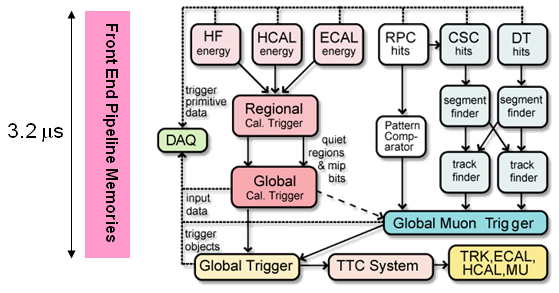
\includegraphics[width=\textwidth]{generated/LoneTrigger/level1trigger.pdf}
  \caption{The CMS \Lone Trigger system}
  \label{fig:figures_LoneTrigger_level1trigger}
\end{figure}


The CMS \Lone trigger system\cite{l1} is a pipelined dead-timeless system based 
on custom-built electronics.
The \Lone trigger is a combination of several sub systems, which are 
interconnected as depicted in 
Figure~\ref{fig:figures_LoneTrigger_level1trigger}.

Corse grain information from the electro-magnetic, hadronic and forward 
calorimeters is processed by the Regional Calorimeter
Trigger (RCT), this is then passed to the Global Calorimeter Trigger (GCT) 
where the corse grain information is clustered in to
physics objects, these objects are then passed to the Global Trigger where the 
\Lone accept decision is made. Due to the limited
size of the pipe line this \Lone accept must be issued within 4.0 $\mu$s.

The objects passed from the GCT to the GT include electro-magnetic objects, 
both electrons and photons as due to the lack of
tracking information at the \Lone trigger these objects are indistinguishable, 
jets and energy sums.

The RCT generates up to 72 isolated and non-isolated electro-magnetic objects, 
these are sorted by rank, which is equivalent to
transverse energy \ET. The four highest ranked electro-magnetic objects are 
then passed via the GCT to the GT at an equivalent data 
rate of 29 \Gbs per type.

Hadronic objects under go two clustering steps. First the transverse energy 
sums of the ECAL and corresponding HCAL towers are
calculated, the towers are then summed in to 4$\times$4 trigger regions, these 
are passed to the GCT at a data rate of 172.8 \Gbs.
These trigger regions are clustered in to jet candidates by the GCT and ranked. 
The jets are then sub-divided in the 
categories depending on their pseudo-rapidity and the result of $\tau$ 
identification. 

Energy sums come in two forms, the total transverse energy \ET which is the 
scalar sum of all transverse energies and the total 
jet transverse energy \HT which is calculated as the scalar sum of all jets 
above some programable threshold.

The missing energy equivalents of these \MET and \MHT are formed from the 
negative vector sum of the objects considered for the
transverse sums.



\section{Leve-1 Trigger Jet Algorithm} % (fold)
\label{sec:leve_1_trigger_jet_algorithm}

\textbf{FIXME: This is taken pretty much straight from \cite{gctcomm} might 
want to steal less??} 

The CMS detector can be un-rolled in the $\phi$ direction to form a rectangular 
grid of the 396 calorimeter regions, connected along the $\phi$ edge. The
rectangle 18 $\phi$ divisions (from $-180^{\circ} < \phi \leq 180^{\circ}$) by 
22 $\eta$ divisions ( from $-5 < \eta < 5$). Each $\phi$ division corresponds 
to 20$^{\circ}$. The $\eta$ divisions correspond to $\Delta\eta$ $= 0.5$ in the 
forward calorimeters and to $\Delta\eta \approx 0.348$ in the barrel.
A pictorial representation of this can be seen in 
figure~\ref{fig:figures_LoneTrigger_jetfindermappings}.

\begin{figure}[ht]
  \centering
    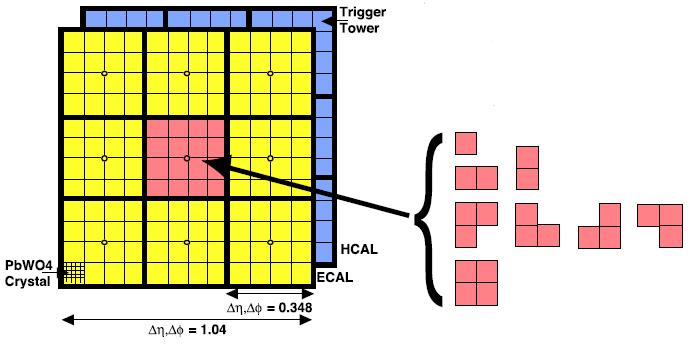
\includegraphics[width=\textwidth]{figures/LoneTrigger/level1jetalgo.jpg}
  \caption{The 3 $\times$ 3 jet-finder window at \Lone. Each cell represents a 
  trigger tower, which is the sum of the HCAL and ECAL transverse energies. The 
  $\tau$-jet veto patterns are shown to the right.}
  \label{fig:figures_LoneTrigger_level1jetalgo}
\end{figure}


A jet candidate is created if the sum of the ECAL and HCAL energies of the 
central calorimeter region has an energy deposit larger than all of its 
neighbours, as shown in figure~\ref{fig:figures_LoneTrigger_level1jetalgo}
The jet is centered at this region where $p_{T}^{central} > p_{T}^{surrounding}$
and the transverse energies of the surrounding regions are summed in to the 
central region. The jet is then classified as a $\tau$ jet if \mETA $< 3.0$ and 
none of the $\tau$ veto bits are set. If any $\tau$ vetoes are set the jet is 
classified as a central jet. The jet is classified as forward if $ 3.0 < \mETA 
< 5.0$

The $\tau$-vetoes are set by the RCT depending on whether or not the energy 
depositions in up to four contiguous trigger towers are below a programmable 
fraction of the regional \ET as shown in 
Figure~\ref{fig:figures_LoneTrigger_level1jetalgo}.

It is possible to apply separate jet energy corrections to each of the sub 
categories of GCT jets. These corrections are discussed in detail in 
Section~\ref{sec:lone_trigger_performance}


\textbf{FIXME: Do we want to add some stuff on the pre-clustering here, i think 
that the answer is yes, but how much?!?!}



\begin{figure}[ht]
  \centering    
  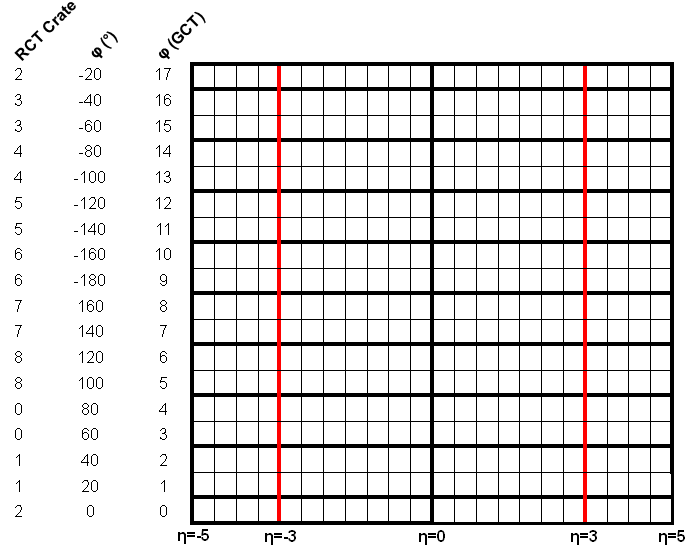
\includegraphics[width=\textwidth]{figures/LoneTrigger/jetfindermappings.png}
  \caption{caption}
  \label{fig:figures_LoneTrigger_jetfindermappings}
\end{figure}




% section leve_1_trigger_jet_algorithm (end)













\section{\Lone Trigger Performance} % (fold)
\label{sec:lone_trigger_performance}

% section lone_trigger_performance (end)

\section{\Lone Trigger Pile-up Mitigation} % (fold)
\label{sub:lone_trigger_pile_up_mitigation}
Due to the lack of a requirement of a jet seed threshold, soft non-collimated 
jets, such as those expected in a high pile up environment are found. Trigger 
decisions are then made using these pile up jets.

This is less of a problem for the single jet triggers which have a high $P_{T}$ 
threshold. However the \HT triggers, where \HT = $\sum_{jets}E_{T}^{jet}$ and 
the requirement of \ET$^{jet} \geq $10 \GeV is made,
see a large increase in rate due to pile-up, this is due to the low energy 
threshold required for a jet to be added to the \HT sum.

To counteract the effect of pile up on trigger rate we study the effects of 
requiring a jet seed threshold on the rate and efficiency of the individual jet 
and \HT triggers.

Figure~\ref{fig:figures_level1jetalgo} depicts 3$\times$3 trigger regions, each 
of which are built from 4$\times$4 trigger towers.
In this case the central region is the jet seed. The proposed change would 
require there to be a threshold energy in the seed region.

The study of using jet seed thresholds of 2 and 5 \GeV is presented. The 
maximum energy of effected jets is 18 \GeV when requiring a seed of 2 \GeV and 
45 \GeV when requiring a seed of 5 \GeV for jets made from $3\times3$ trigger 
regions, however some jets can include more than 9 trigger regions. The jet 
clustering is performed before the \Lone jets are corrected according 
to their \ET and $\eta$, hence the effects are manifested in trigger decisions 
for \Lone jets above 18 or 45 \GeV.



\begin{figure}[h!]
    \centering
    \subfigure[GCT jet $E_{T}$ distributions for the same events with a 0, 2 or 5 \GeV seed requirement.]{
          \label{fig:GCTrankRAW}
          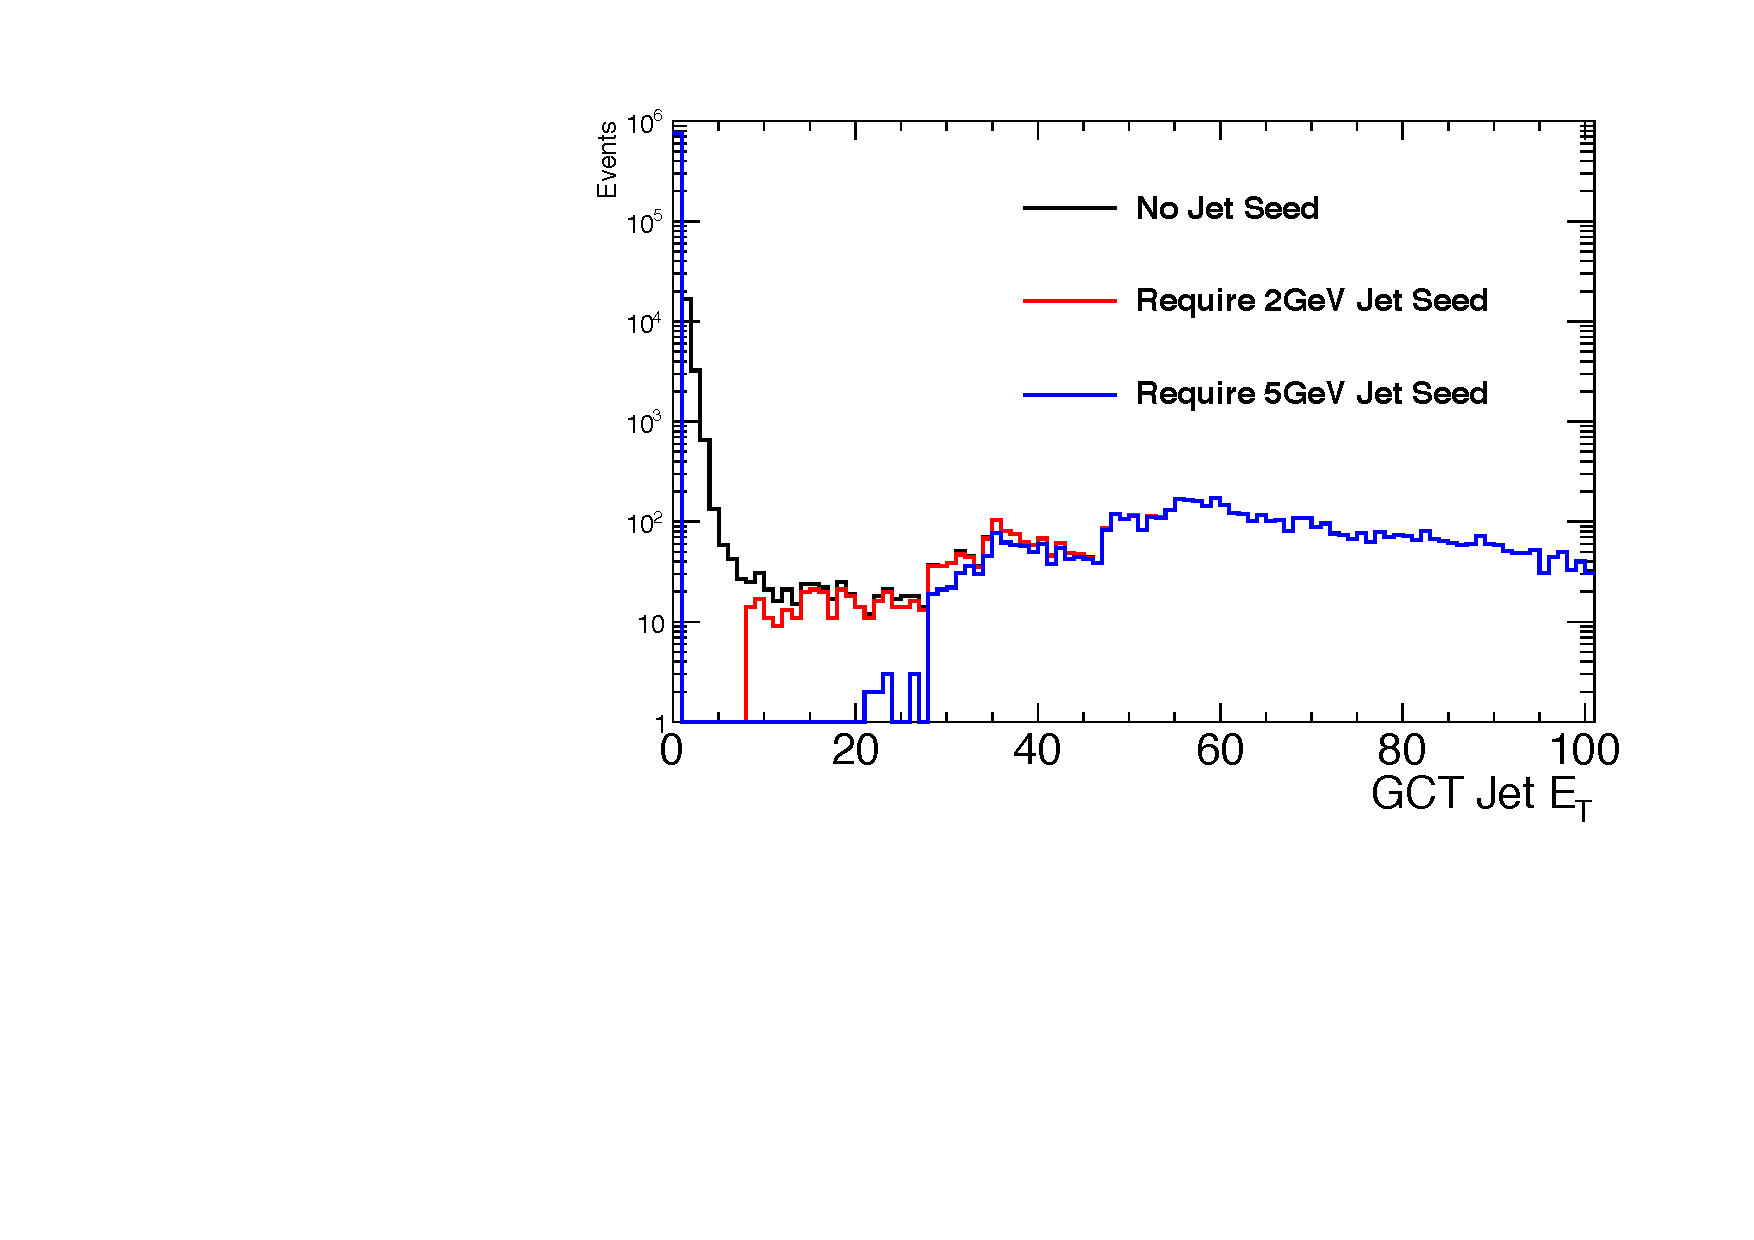
\includegraphics[width=0.45\textwidth]{generated/LoneTrigger/GCT_Jet_Rank_highPU.pdf}
     }
    \subfigure[Efficiency of applying a requirement of 2 or 5 \GeV with respect to no requirement.]{
          \label{fig:GCTrankRatio}
          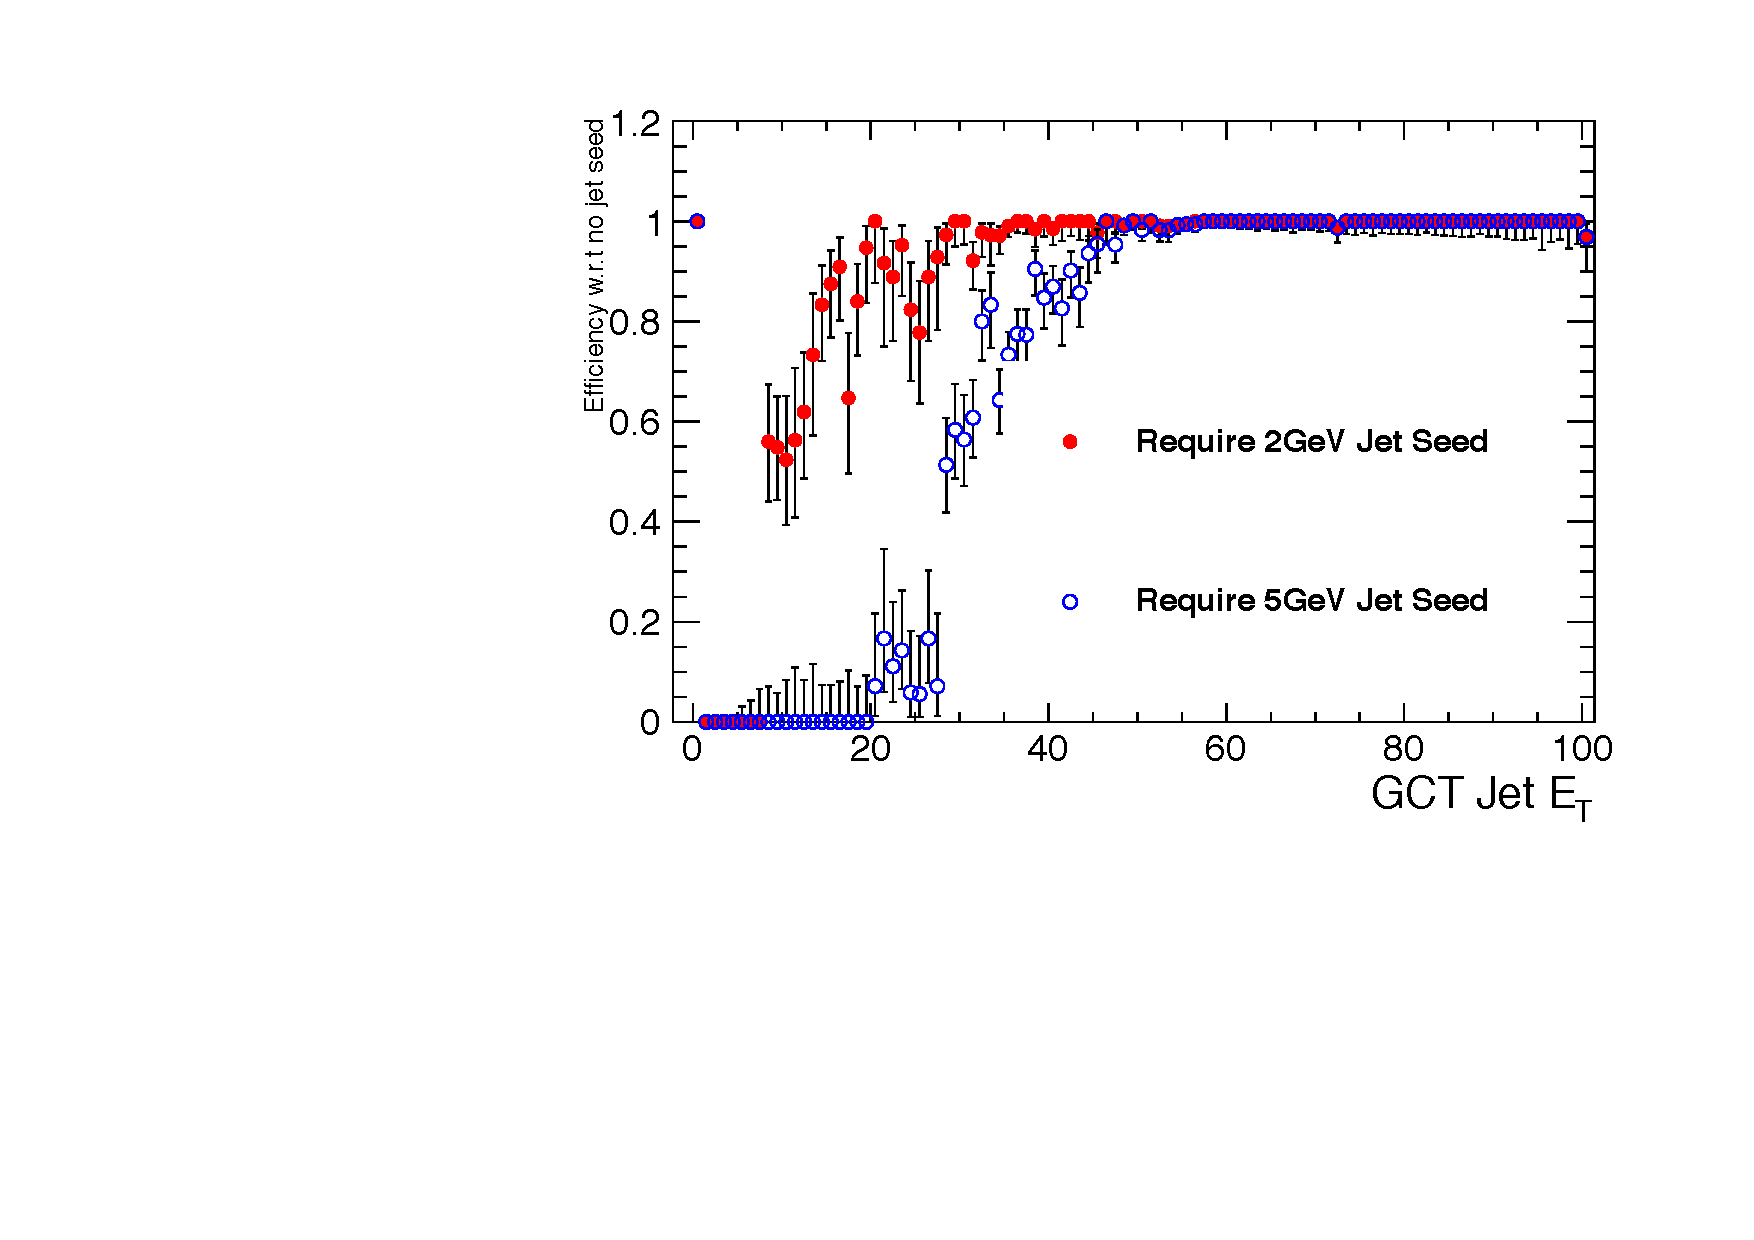
\includegraphics[width=0.45\textwidth]{generated/LoneTrigger/GCT_Jet_Rank_highPU_ratio.pdf}
     }
    \caption{Effect of requiring a jet seed threshold on GCT internal jets.}
    \label{fig:GCTrank}
\end{figure}


Figure~\ref{fig:GCTrank} shows how the different threshold requirements effect 
the rank of the internal GCT jets. The effect is to remove all jets below 
2(5)\GeV and to cut out jets from the low end of the distribution. From 
Figure~\ref{fig:GCTrankRatio} it is possible to see the point beyond which the 
requirement of a jet seed has no effect. For a cut of 2 \GeV jets above a rank 
of $\approx$ 35 are not effected, for a seed threshold of 5 \GeV jets above a 
rank of 55 are not effected.


\begin{figure}[ht]
  \centering
    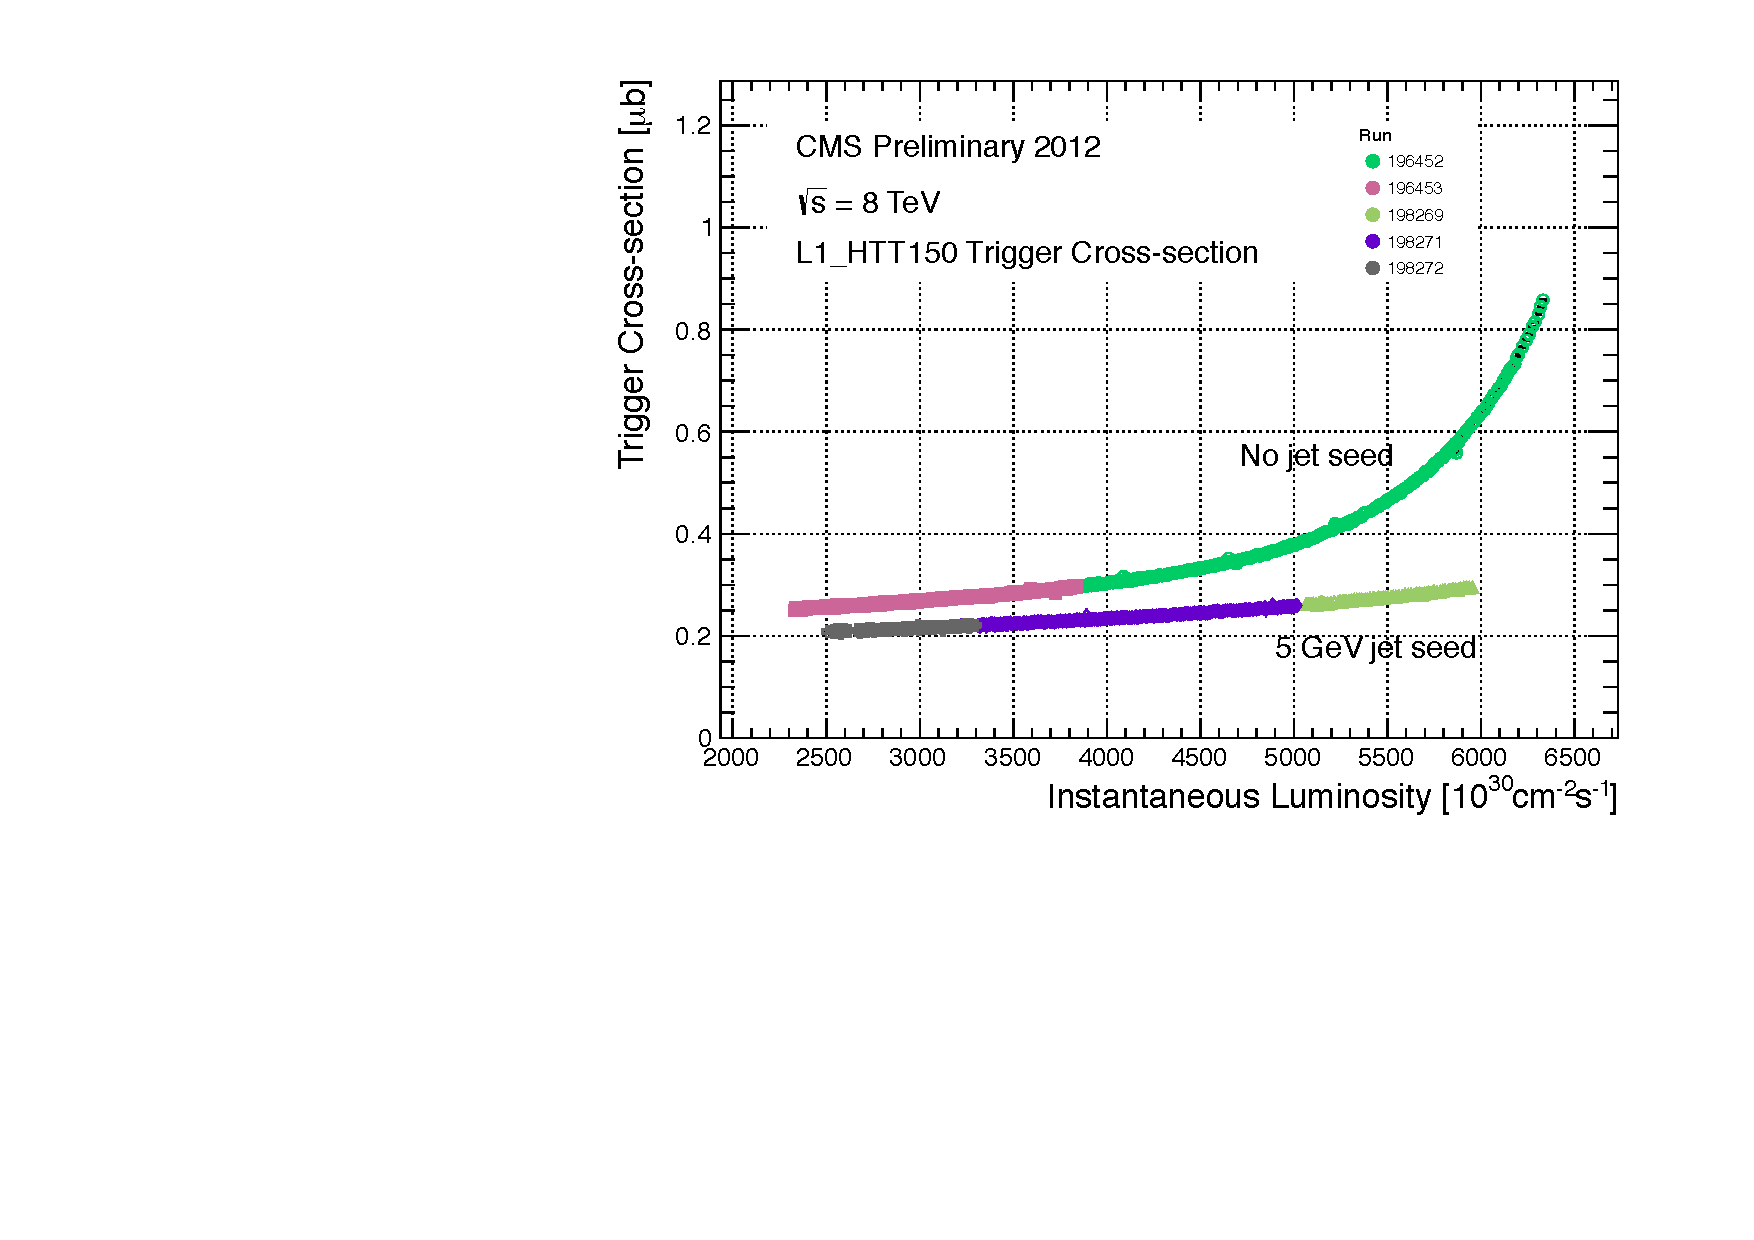
\includegraphics[width=\textwidth]{figures/LoneTrigger/HTT150_pileup.pdf}
  \caption{caption}
  \label{fig:figures_LoneTrigger_HTT150_pileup}
\end{figure}


% subsection lone_trigger_pile_up_mitigation (end)


% chapter level_one_trigger (end)